\RequirePackage[l2tabu, orthodox]{nag}
\documentclass[a4paper, twocolumn]{article}
\usepackage[utf8]{inputenc}
\usepackage[T1]{fontenc}
\usepackage[pdftex, hidelinks,
            pdftitle={Behaviour Tree Evolution by Genetic Programming},
            pdfauthor={Martin Estgren and Erik S. V. Jansson},
            pdfsubject={Artificial Intelligence - Genetic Programming},
            pdfkeywords={artificial intelligence, genetic programming,
                         behaviour trees, a-star, shooter}]{hyperref}

\usepackage{bm}
\usepackage{caption}
\usepackage{listings}
\usepackage{booktabs}
\usepackage{mathtools}
\usepackage{algorithmic}
\usepackage{graphicx}
\usepackage{courier}
\usepackage{amsmath}
\usepackage{amssymb}
\usepackage{algorithm}
\usepackage[capitalize, noabbrev]{cleveref}
\usepackage[activate={true, nocompatibility}, final,
            tracking=true, kerning=true, spacing=true,
            factor=1100, stretch=10, shrink=10]{microtype}

\newcommand\blfootnote[1]{%
    \begingroup
        \renewcommand\thefootnote{}\footnote{#1}%
        \addtocounter{footnote}{-1}%
    \endgroup
}

\DeclareCaptionFormat{modifiedlst}{\rule{\textwidth}{0.85pt}\\[-2.9pt]#1#2#3}
\captionsetup[lstlisting]{format =  modifiedlst,
labelfont=bf,singlelinecheck=off,labelsep=space}
\lstset{basicstyle=\footnotesize\ttfamily,
        breakatwhitespace = false,
        breaklines = true,
        keepspaces = true,
        language = Java,
        showspaces = false,
        showstringspaces = false,
        frame = tb,
        numbers = left,
        numbersep = 5pt,
        xleftmargin = 16pt,
        framexleftmargin = 16pt,
        belowskip = \bigskipamount,
        aboveskip = \bigskipamount,
        escapeinside={<@}{@>}}

\title{\textbf{Behaviour Tree Evolution by Genetic Programming}\\
       \Large{\emph{-- Learning Novel Bot Behaviours in a 2D Top-Down Arena Shooter --}}}
\author{{\textbf{Martin Estgren}} \;\;\;\;\;\;\;\;\;\, {\href{mailto:mares480@student.liu.se}
                                                       {\texttt{<mares480@student.liu.se>}}} \\
        {\textbf{Erik S. V. Jansson}} \;\;\;\;         {\href{mailto:erija578@student.liu.se}
                                                       {\texttt{<erija578@student.liu.se>}}} \\~\\
        {Linköping University, Sweden}\vspace{-2.0ex}}

\begin{document}
    \maketitle
    \section*{Abstract}

    Behaviour trees are a popular model for representing the decision-making and plan execution process for NPCs in video games. These are built by hand, and require expertise to craft. They don't adapt well to other environments, and often require a custom BT.

    In this paper we demonstrate how to generate the BTs by using genetic programming; allowing us to essentially evolve novel behaviours automatically in our testbed. Instead of specifying low-level actions and conditions, we use high-level definitions. This leads to faster fitness convergence, and also allows us to skip the bloat control and tree pruning steps used by other methods. Results show that the evolved BT beats our hand-crafted BT by the \(5^{th}\) generation. \footnotemark[1]

    \vspace{1.0em}

    \begingroup
    \def\addvspace#1{}
    \tableofcontents
    \endgroup
    \newpage

    \newpage % Next column...
    \nocite{*} % Include all.
    \bibliographystyle{abbrv}
    \bibliography{report}
    \footnotetext[1]{Repository: \url{https://github.com/sci10n/Quake2D}}
    \clearpage

    \section{Introduction} \label{sec:introduction}

    In interactive media such as games, there is often a need for simulating seemingly complex agent behaviours in real-time. In modern fast-paced computer games for example, the render, physics and artificial intelligence steps all need to complete in a total of less than 16ms to provide a half-decent experience. These requirements have spawned some clever techniques to enable complex behaviours for autonomous agents, while keeping their computation time short.

    These techniques often require manual behaviour definition, and in some cases, are hard to extend when new behaviours are needed for a game, as shown by industry researchers, e.g. \emph{Dawe et al}~\cite{dawe2014overview}, regarding the finite state machine architecture. In this project we have explored how one of the more widely used techniques, \emph{behaviour trees}, can be extended to allow for not only hand-crafted complex behaviors, but for organic behaviours tailored to the specific game domain by using \emph{reinforcement learning}. More specifically, we evolve behaviour trees with \emph{genetic programming}, which spawn behaviour tree offspring.

    Alongside the proposed method in \cref{sec:proposed_approach}, a testbed consisting of a top-down arena shooter was built. It features a sufficiently complex environment to support interesting behaviours by the enemy bot. We describe the features of our testbed in \cref{sec:implementation_details}.

    This report starts off in \cref{sec:background_theory} by giving a brief overview of the relevant techniques and related work necessary to follow our reasoning and findings. In \cref{sec:implementation_details} we describe the details needed to implement these techniques in practice, along with the testbed architecture we've used. This gives the reader information on any peculiarities and pit-falls. We follow this by showing in \cref{sec:results_and_screenshots} the testbed, and give some generated offspring generated by our method along with measurements of its efficiency. Finally, we reflect on our method, giving downsides, and present some possible future work in \cref{sec:discussion_and_outlook}.

    \vspace{-0.8em}

    \subsection{Proposed Approach} \label{sec:proposed_approach}

    Apply \emph{genetic programming} to the \emph{behaviours trees} by creating \emph{high-level actions and conditions} nodes. Ideally this should allow for faster convergence rates and somewhat shallower generated behaviour trees, eliminating the need for bloat control and pruning. Since BTs are trees, the \emph{mutation mechanism} should modify \emph{control-flow structure} and \emph{leaf-node settings}, while the \emph{crossover mechanism} will swap sub-trees.

    \section{Background Theory} \label{sec:background_theory}

    For an autonomous agent to give the illusion of intelligence, many different systems and techniques need to interact with each other. In this chapter we describe the theory behind our three primary systems: \emph{behaviour trees}, \emph{path finding} \& \emph{genetic programming}.

        \subsection{Behaviour Trees} \label{sec:behaviour_trees}

        Defining an accurate \emph{automatic planner} model is often impractical and usually overkill for real-world applications. Especially in games, where very simple models are enough to give the illusion of intelligence. In games, the most well-known \emph{behaviour selection algorithms} are \emph{FSMs}, \emph{GOAPs}, \emph{HTNs} and \emph{BTs} \cite{dawe2014overview}.

        \emph{Finite State Machines (FSMs)} are simple but are hard to extend with additional states, making the amount of transitions to be specified to blow up \cite{dawe2014overview}. While both \emph{GOAP (Goal-Oriented Action Planner)} and \emph{HTN (Hierarchical Task Network)} are powerful models, these don't allow agents to explore new task definitions, and ``only'' provide an agent with novel ways of solving an already defined set of task defs.

        \emph{Behaviour Trees (BTs)} on the other hand, when comparing to FSMs, provide advantages in terms of modularity, reactiveness and scalability. And more importantly, since they are a type of tree, allow for integration with the genetic programming approach. They were first popularized by the game \emph{Halo 2}, but are now used in other area as well, such as robotics.

        In the \emph{Behaviour Tree Starter Kit}~\cite{champandard2014behaviour} and also in \emph{Chris Simpson's Gamasutra article}~\cite{simpson2014behavior}, the BT is a tree-like data structure which describes the decision-making process of the agent. It's evaluated pre-order from the root of the tree in each logic update tick.

        \begin{figure}[H]
            \centering
            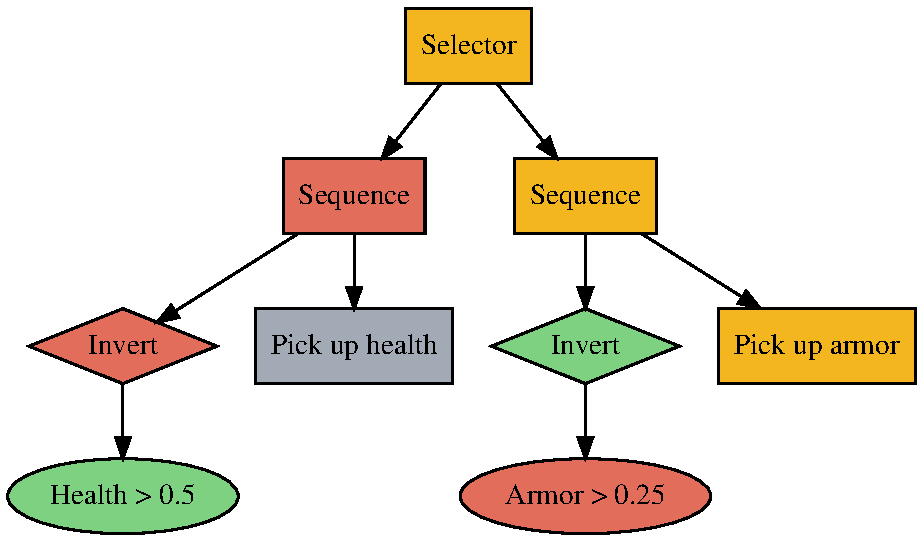
\includegraphics[width=\linewidth]{share/behaviour_tree.pdf}
            \caption{Example of Hand-Crafted Behaviour Tree}
            \label{fig:behaviour_tree}
        \end{figure}

        Below you'll find the most common types of nodes in a behaviour tree, such as those specified in \emph{Behaviour Tree Starter Kit}~\cite{champandard2014behaviour} and \emph{Simpson's paper}~\cite{simpson2014behavior}. \emph{Selectors} and \emph{sequences} are \emph{composite control-flow nodes} which order and choose the children to run. \emph{Inverters} and \emph{succeeder} are \emph{decorator nodes} which modify the result of a leaf node. Finally, \emph{action and condition nodes} are \emph{leaf-nodes} which can either be \emph{running}, \emph{failed} or \emph{succeeded}. The states of these nodes propagates upwards in the tree.

        \begin{itemize}
            \item{\textbf{Selector:} executes children from left \(\rightarrow\) right until \emph{one child} is found to be either \emph{running} or has already \emph{succeeded}, and returns this status. Otherwise, it if none match, it returns a \emph{failure}.}
            \item{\textbf{Sequence:} executes children from left \(\rightarrow\) right until \emph{one child} is found to be either \emph{running} or \emph{failed}, and returns this status. If \emph{all children} have \emph{succeeded}, then also set status to \emph{success}.}
            \item{\textbf{Parallel Selector/Sequence:} similar to the above, but executes \emph{all children simultaneously}.}
            \item{\textbf{Inverter:} executes the child node and \emph{inverts the resulting state} when it has finished running.}
            \item{\textbf{Succeeder:} when child has finished running, returns \emph{success} regardless of the child's status.}
            \item{\textbf{Condition:} a leaf-node that queries the world state, if the query returns true, we give \emph{success}, if it's false, we instead give \emph{failure}. This node is usually instantaneous, and can't be \emph{running}.}
            \item{\textbf{Action:} a leaf-node which modifies the world state, and returns \emph{success} if the action had the intended side-effect, \emph{failure} if couldn't complete or failed the action and \emph{running} if not done yet.}

        \end{itemize}

        We find that it's easier to understand behaviour trees with an example. Look back at \cref{fig:behaviour_tree}. It's a sub-tree of the hand-crafted BT we produced for our testbed. Yellow represents \emph{running} nodes, green have \emph{succeeded} and red have \emph{failed}. First we enter the root node, the selector, which will in run its child nodes in order until one has succeeded. In this case the first child fails because the sub-tree of that child failed. The other sub-tree hasn't yet terminated with either succeed or fail, and the agent is currently trying to pick up armour.

        \subsection{Path Finding with A*} \label{sec:path_finding}

	Agent path finding is done using the \emph{A*} graph traversal algorithm proposed by Peter E. Hart, Nils J. Nilsson, and Bertram Raphael ~\cite{hart1968formal} as an extension to \emph{Dijkstra's algorithm} which, given an \emph{admissible heuristic} and non-negative costs, will find the path from a node \(n_0\) to node \(n_g\) with the lowest cost.
	
	Calculating the expected cost of an path from \(n_0,...,n_k,...,n_g\) can be done as the following function:
	\begin{equation*}
		f(n_k) = g(n_k) + h(n_k)
	\end{equation*}	
	where \(g(n_k)\) is the true cost from \(n_0\) to node \(n_k\) and \(h(n_k)\) is a heuristic approximation of the cost from \(n_k\) to \(n_g\).

        In this project, \emph{euclidean distance} is used as the heuristic \(h(n_k)\) since the path-finding is performed in a search-space where each node is defined as a point in the world-space. 

	Additionally to regular \emph{A*}, the pathfinder also utilizes an \emph{influence map} to help the agent avoid suicidal paths, even if the selected path is optimal given the heuristic function. The \emph{influence map} takes into account the visibility of each node in relation to adversarial game agents' line-of-sight and updates the expected cost as:
	\begin{equation*}
		f(n_k) = g(n_k) + h(n_k) + i(n_k)
	\end{equation*} 
	which has the result of nodes within adversarial agents line-of-sight having a much higher associated traversal cost. 
	
\begin{minipage}{\linewidth}        	
        \centering
	\begin{minipage}{0.4\linewidth}
	\begin{figure}[H]
		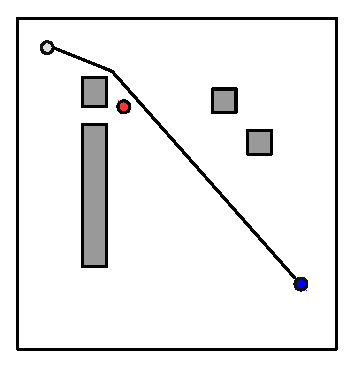
\includegraphics[width=\linewidth]{share/bad.eps}
		\caption{}
		\label{fig:optimal_path}
        \end{figure}
	\end{minipage}
	\hspace{0.05\linewidth}
	\begin{minipage}{0.4\linewidth}
	\begin{figure}[H]
		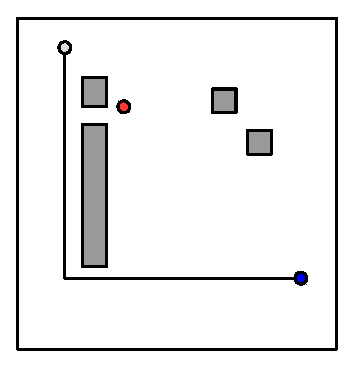
\includegraphics[width=\linewidth]{share/good.eps}
		\caption{}
		\label{fig:smart_path}
	\end{figure}
	\end{minipage}
\end{minipage}
	Above are two example figures, one showing (fig~\ref{fig:optimal_path}) an optimal path using regular \emph{A*}, and the other showing the optimal path when taking into account the influence map (fig~\ref{fig:smart_path}).
	
	\subsection{Genetic Programming} \label{sec:genetic_programming}

	In many scenarios you try to optimize the input of an function \(f(x_0,x_1,...,x_n)\) where some or all of the inputs are of an discrete nature (ordinal or nominal values). These types of problems are often hard to optimize using techniques developed for continuous variables, such as \emph{gradient ascent/descent}.

	\emph{Genetic programming} is an technique presented by \emph{Nils Barricelli} ~\cite{barricelli1954esempi} as a way to optimize computer programs by encoding with \emph{genetic representation} which could be processed by \emph{evolutionary algorithms}. 

	\begin{figure}[H]
		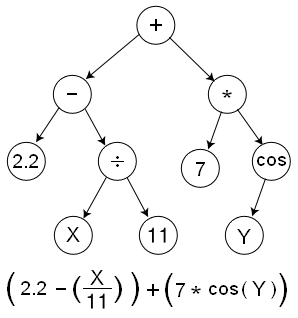
\includegraphics[width=0.8\linewidth]{share/Genetic_Program_Tree.png}
		\caption{The \emph{genetic representation} is often done using a tree structure in \emph{genetic programming}.}
		\label{fig:genetic_representation}
	\end{figure}

	The typical \emph{evolutionary algorithm} can be described in the following steps:
    \begin{enumerate}
        \item Generate initial population - Create a pool \(\mathcal{P_0}\) of individuals with randomized genetic representations.
        \item Evaluate \emph{fitness} for each individual \(x_i\) - this usually requires a domain specific \emph{fitness function} \(f(x_i)\rightarrow f_i \in \mathbf{R}\), which will be described in further detail later in this section.
        \item Remove individuals with poor \textit{low fitness score} and \emph{regenerate} the population pool.
    \end{enumerate}

    The \emph{fitness function} for this project is an \emph{linear combination} of desirable behaviours collected during the \emph{Fitness evaluation} simulation such as \emph{damage dealt} to adversary, whether the agent with a specific BT \emph{survived}, and how many \emph{weapons the agent picked-up}. 

	\emph{Regeneration} of the population pool for the next generation \(\mathcal{P}_{t+1}\) is done using three functions:

    \textbf{Select} ~ \(\Phi_s(\mathcal{P}_t) \rightarrow x_i \in \mathcal{P}_t\) individuals with high \emph{fitness score}. In this project, \emph{selection} is done proportionally to the \emph{fitness score} for each individual. Each individual \(x_i\) has a probability \(P(x_i|f_i)\) to be selected for the next generation \(\mathcal{P}_{t+1}\):
    \begin{equation*}
        P(x_i|f_i) = \frac{f_i}{\sum_{j = 1}^{N}f_j}
    \end{equation*}
    where \(N = |\mathcal{P}_t|\)

    \textbf{Crossover} ~ \(\Phi_c(x_i,x_j) \rightarrow \hat{x_i},\hat{x_j}\) individuals from the new population, in the case of \emph{genetic programming}, crossover is done by swapping random \emph{sub-trees} in each BT. All sub-tree has an equal probability of being selected for \emph{crossover}

    \textbf{Mutate} ~ \(\Phi_m(x_i) \rightarrow \hat{x_i}\) a subset of the new population, slightly tweaking a random parameter or adding/removing a random child node. Once these steps have been performed, a new generation of individuals have been produced which can repeat the optimization process until we reach converge to a population of \emph{behaviours} close the global maximum of the fitness function.

	
    \section{Implementation Details} \label{sec:implementation_details}



        \subsection{Game Architecture} \label{sec:game_architecture}


        \subsection{Behaviour Trees} \label{sec:behaviour_trees_implementation}


        \subsection{Genetic Programming} \label{sec:genetic_programming_implementation}



    \section{Results and Screenshots} \label{sec:results_and_screenshots}



        \subsection{Generated Behaviours} \label{sec:generated_behaviours}



        \subsection{Behaviour Fitness} \label{sec:behaviour_fitness}



        \subsection{Survival Rate} \label{sec:survival_rate}



    \section{Discussion and Outlook} \label{sec:discussion_and_outlook}



\end{document}
